\documentclass[10pt,twocolumn]{extarticle}
\usepackage[a4paper,margin=1.5cm,columnsep=0.7cm]{geometry}
\usepackage{amsmath,amssymb}
\usepackage{graphicx}
\usepackage{enumitem}
\usepackage{booktabs}
\usepackage{array}
\usepackage{tabularx}
\usepackage[T1]{fontenc}

\setlength{\parindent}{0pt}
\setlength{\parskip}{4pt}
\renewcommand{\arraystretch}{1.15}

\newenvironment{qoptions}{\begin{itemize}[leftmargin=1.8em,itemsep=2pt,topsep=2pt,label={}]}{\end{itemize}}
\newcommand{\opt}[2]{\item[({#1})] {#2}}

\newcommand{\sectionhdr}[1]{\par\vspace{4pt}\noindent\textbf{\large #1}\par\vspace{2pt}}
\newcommand{\subsectionhdr}[1]{\par\vspace{3pt}\noindent\textbf{#1}\par\vspace{2pt}}

\pagestyle{empty}

\begin{document}
\twocolumn[
\begin{center}
{\LARGE\bfseries JEE (Main+Advanced) Score-II --- Test 18 (13 Feb 2024)}
\end{center}
\vspace{6pt}
]

\sectionhdr{PART-1: PHYSICS}
\subsectionhdr{Section-I (i): Single Correct}

\textbf{1.} A hemispherical shell of mass M is kept on a rough horizontal surface as shown. An insect of mass m starts traveling up from the bottom very slowly. There is no slipping between the ground and the hemisphere. The minimum coefficient of friction between the inner surface of the shell and the insect so that it can reach the edge of the hemisphere is:

\begin{center}
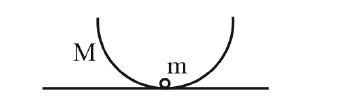
\includegraphics[width=0.55\linewidth]{Score-II - Test 18 (13 Feb 2024)-img/p1phy_q1_hemisphere.png}
\end{center}

\begin{qoptions}
\opt{A}{$\mu \geqslant \dfrac{M}{2m}$}
\opt{B}{$\mu \geqslant \dfrac{M}{3m}$}
\opt{C}{$\mu \geqslant \dfrac{3M}{2m}$}
\opt{D}{$\mu \geqslant \dfrac{M}{4m}$}
\end{qoptions}

\textbf{2.} Two particles of mass m each are kept on a horizontal circular platform on two mutually perpendicular radii at equal distance r from the centre of the table. The particles are connected with string, which is just taut when the platform is not rotating coefficient of static friction between the platform and particle is $\mu$. The maximum angular speed ($\omega$) of platform about its centre so that the particle remain stationary relative to platform is

\begin{center}
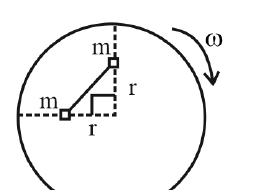
\includegraphics[width=0.42\linewidth]{Score-II - Test 18 (13 Feb 2024)-img/p1phy_q2_platform.png}
\end{center}

\begin{qoptions}
\opt{A}{$\sqrt{\dfrac{\sqrt3\,\mu g}{r}}$}
\opt{B}{$\sqrt{\dfrac{\sqrt2\,\mu g}{r}}$}
\opt{C}{$\sqrt{\dfrac{\sqrt5\,\mu g}{r}}$}
\opt{D}{None}
\end{qoptions}

\textbf{3.} A sonic source with frequency 1000 Hz and a receiver are located at the same point. At t = 0 both (source and receiver) start receding each other with constant acceleration 1.25 m/s$^2$ and 12 m/s$^2$ respectively. Find the approximate frequency detected by the receiver after 10s. Take velocity of sound v = 320 m/s.

\begin{qoptions}
\opt{A}{450 Hz}
\opt{B}{700 Hz}
\opt{C}{500 Hz}
\opt{D}{600 Hz}
\end{qoptions}

\textbf{4.} A stable species C can be obtained through unstable nuclides A and B. The half life period for conversion A $\to$ C is T and that for conversion B $\to$ C is 2T. Initially a sample contains N nuclides of A, N nuclides of B and no nuclides of C. After how much time will the nuclides of species C be equal to (27/16) N

\begin{qoptions}
\opt{A}{2T}
\opt{B}{3T}
\opt{C}{4T}
\opt{D}{5T}
\end{qoptions}

\textbf{5.} In a single slit diffraction experiment, two tungsten plates P$_1$ and P$_2$ are mounted on two rigid walls close to each other to make a slit. Length of each plate is 2.5 cm at 20$^\circ$C. At the temperature of 50$^\circ$C the point on the screen previously occupied by fourth minima of wavelength $\lambda_1=5000\,\text{\AA}$ is now occupied by second minima of $\lambda_2=7000\,\text{\AA}$. At temperature of 90$^\circ$C angular position fifth minima of $\lambda_3=6000\,\text{\AA}$ is found to be $30^\circ$. Mark the correct statement(s)

\begin{center}
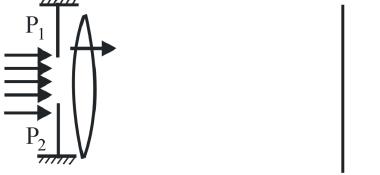
\includegraphics[width=0.45\linewidth]{Score-II - Test 18 (13 Feb 2024)-img/p1phy_q5_slit.png}
\end{center}

\begin{qoptions}
\opt{A}{The coefficient of linear expansion $\alpha$ of plates is $4\times10^{-6}$/K}
\opt{B}{The coefficient of linear expansion $\alpha$ of plates is $5\times10^{-6}$/K}
\opt{C}{The coefficient of linear expansion $\alpha$ of plates is $3\times10^{-6}$/K}
\opt{D}{The coefficient of linear expansion $\alpha$ of plates is $6\times10^{-6}$/K}
\end{qoptions}

\textbf{6.} An infinitely long cylindrical wire of radius 'R' is carrying a current with current density j = $\alpha r^3$ (where $\alpha$ is constant and 'r' is the radial distance from the axis of the wire). If the magnetic field at r = $\dfrac{R}{2}$ is 'B$_1$' and at r = 2R is 'B$_2$' then the ratio $\dfrac{B_2}{B_1}$ is

\begin{qoptions}
\opt{A}{2}
\opt{B}{4}
\opt{C}{6}
\opt{D}{8}
\end{qoptions}

\subsectionhdr{Section-I (ii): One or more correct}

\textbf{7.} A drop of liquid of volume V is squeezed between two parallel smooth plates unit the liquid thickness h is very small compared with the liquid's radial extent R. The liquid/plate/air contact angle $\alpha$, and the liquid/air surface tension is $\sigma$. Gravitational effects are negligible.

\begin{center}
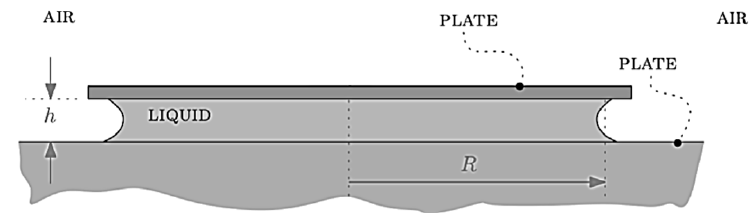
\includegraphics[width=0.95\linewidth]{Score-II - Test 18 (13 Feb 2024)-img/p1phy_q7_liquid.png}
\end{center}

\begin{qoptions}
\opt{A}{If $\alpha\simeq0$, then pressure inside liquid will be lesser by $\left(\dfrac{2\sigma}{h}\right)$ as compared to P$_{atm}$.}
\opt{B}{If $\alpha\simeq0$, then pressure inside liquid will be more by $\left(\dfrac{2\sigma}{h}\right)$ compared to P$_{atm}$.}
\opt{C}{If upper plate is massless then upward force required to hold the plate in equilibrium will be approximately $\sigma 2\pi R\sin\alpha + \left(\dfrac{2\sigma}{h}\right)\pi R^2\ (0<\alpha<90)$}
\opt{D}{If upper plate is massless then upward force required to hold the plate in equilibrium will be approximately $\sigma 2\pi R\sin\alpha - \left(\dfrac{2\sigma}{h}\right)\pi R^2\ (0<\alpha<90)$}
\end{qoptions}

\textbf{8.} Lets try calculating the power of turbine. Water turbine consists of large number of paddles that could be considered as light slat boards [see fig] with length $\ell$, are at one end attached to rotating axis. A stream of water with velocity v and flow rate $\mu$ kg/s with respect to ground is directed on turbine such that it only hits edges of paddles. [assume that water comes to rest with respect to paddle just after hitting plates and number of blades are large]

\begin{center}
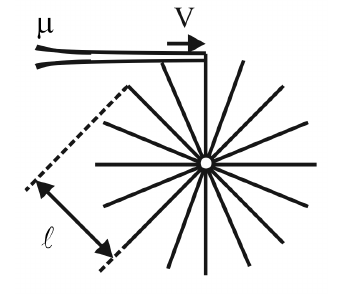
\includegraphics[width=0.5\linewidth]{Score-II - Test 18 (13 Feb 2024)-img/p1phy_q8_turbine.png}
\end{center}

Choose the correct option(s)

\begin{qoptions}
\opt{A}{Maximum possible power that can be extracted from turbine is at angular velocity $\dfrac{v}{2\ell}$ of blades.}
\opt{B}{Maximum possible power that can be extracted from turbine is at angular velocity $\dfrac{v}{3\ell}$ of blades.}
\opt{C}{Maximum power supplied to turbine will be $\dfrac{8}{27}$ of kinetic energy of incoming liquid per unit time}
\opt{D}{Maximum power supplied to turbine will be $\dfrac{8}{9}$ of kinetic energy of incoming liquid per unit time}
\end{qoptions}

\textbf{9.} A (suitably made) wire coat hanger can perform small amplitude oscillation in the plane of the figure around the equilibrium positions shown. In positions (a) and (b) the long side is horizontal. The other two sides have equal length. The period of oscillation is the same in all cases.

\begin{center}
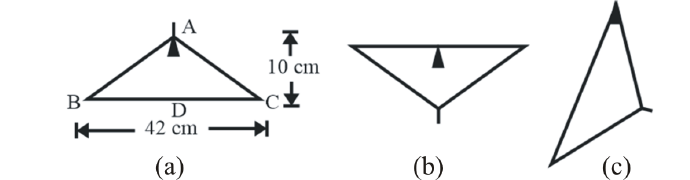
\includegraphics[width=0.95\linewidth]{Score-II - Test 18 (13 Feb 2024)-img/p1phy_q9_hanger.png}
\end{center}

The figure does not contain any information beyond the dimensions given. Nothing is known, e.g., concerning the detailed distribution of mass.

\begin{qoptions}
\opt{A}{Center of mass must be somewhere on AD line [D is mid point of BC]}
\opt{B}{Time period of oscillation will be $2\pi\sqrt{\dfrac{\left(\frac{d_1^2}{4}+\frac{d_2^2}{4}\right)^{1/2}+\frac{d_2}{2}}{g}}$ \{Here BC = d$_1$, AD = d$_2$\}}
\opt{C}{Time period of oscillation will be $2\pi\sqrt{\dfrac{\left(\frac{d_1^2}{4}+\frac{d_2^2}{4}\right)^{1/2}+\frac{d_2}{4}}{g}}$ \{Here BC = d$_1$, AD = d$_2$\}}
\opt{D}{Center of mass of hanger can not be on line AD}
\end{qoptions}

\textbf{10.} A non conducting ring of radius R and charge Q [uniformly distributed] is fixed in gravity free space. A particle of m and magnitude of charge q is placed at the centre of ring. [ignore gravity]. $\left(k=\dfrac{1}{4\pi\varepsilon_0}\right)$

\begin{center}
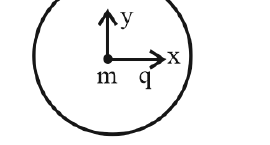
\includegraphics[width=0.35\linewidth]{Score-II - Test 18 (13 Feb 2024)-img/p1phy_q10_ring.png}
\end{center}

\begin{qoptions}
\opt{A}{If particle (Negatively charged) is displaced by ($\delta\to0$) out of plane along z axis and released. Its time period of oscillation will be $2\pi\sqrt{\dfrac{mR^3}{kQq}}$}
\opt{B}{If particle (Negatively charged) is displaced by ($\delta\to0$) out of plane along z axis and released. Its time period of oscillation will be $2\pi\sqrt{\dfrac{2mR^3}{kQq}}$}
\opt{C}{If particle (Positively charged) is displaced by ($\delta\to0$) in the plane of ring along x axis and released. Its time period of oscillation will be $2\pi\sqrt{\dfrac{2mR^3}{kQq}}$.}
\opt{D}{If particle (Positively charged) is displaced by ($\delta\to0$) in the plane of ring along x axis and released. Its time period of oscillation will be $2\pi\sqrt{\dfrac{mR^3}{4kQq}}$}
\end{qoptions}

\textbf{11.} System shown in figure is in steady state. Capacitor shown is filled with di-electric constant (k = 2) and capacitance of capacitor with di-electric is 6$\mu$F. Now at t = 0, di-electric is suddenly removed choose the correct options.

\begin{center}
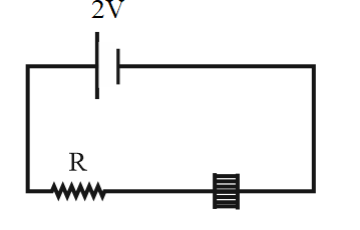
\includegraphics[width=0.5\linewidth]{Score-II - Test 18 (13 Feb 2024)-img/p1phy_q11_circuit.png}
\end{center}

\begin{qoptions}
\opt{A}{Charge on the capacitor just after removal of de-electric is 6$\mu$c.}
\opt{B}{Charge on the capacitor just after removal of de-electric is 12$\mu$c.}
\opt{C}{Heat generated in resistor ($0<t<\infty$) is 2 $\mu$J}
\opt{D}{Heat generated in resistor ($0<t<\infty$) is 6 $\mu$J}
\end{qoptions}

\textbf{12.} A rectangular loop of width b, length $\ell$, mass m and resistance R is placed close to and coplanar with a very long fixed straight conductor carrying current I. One side of the loop is parallel to the straight conductor as shown in the figure. The current in the conductor is suddenly switched off. Neglecting gravity

\begin{center}
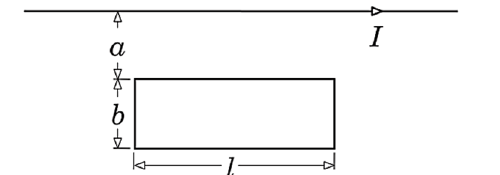
\includegraphics[width=0.55\linewidth]{Score-II - Test 18 (13 Feb 2024)-img/p1phy_q12_loop.png}
\end{center}

\begin{qoptions}
\opt{A}{Velocity acquired by loop is $\dfrac{\mu_0^2\,b\,\ell^2\,I^2}{8\pi^2 mRa(a+b)}\ell n\left(\dfrac{a+b}{a}\right)$.}
\opt{B}{Velocity acquired by loop is $\dfrac{\mu_0^2\,b\,\ell^2\,I^2}{4\pi^2 mRa(a+b)}\ell n\left(\dfrac{a+b}{a}\right)$.}
\opt{C}{Loop will acquire velocity towards the wire.}
\opt{D}{Loop will acquire velocity away from the wire}
\end{qoptions}

\subsectionhdr{Section-II: Numerical Value}

\textbf{1.} Two balls of unequal masses, moving in opposite directions with equal speeds collide elastically. Thereafter, the heavier particle is observed deviated from its original direction of motion by an angle $\alpha=30^\circ$ in the laboratory frame and by an angle $\beta=60^\circ$ in the centre of mass frame. Find the ratio of heavier mass to lighter mass.

\textbf{2.} Consider the arrangement as shown in the figure. A uniform wire (linear mass density 0.2 g/m) vibrating in its fundamental mode is in resonance with air column in a resonance tube vibrating in 1$^{st}$ overtone. The value of m is $\dfrac{54}{K}$kg. Find the value of k. (Given that speed of sound in air is 400 m/s and g = 10 m/s$^2$)

\begin{center}
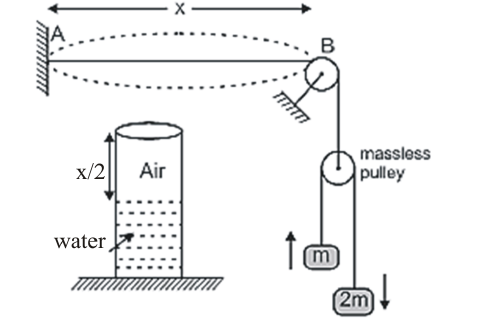
\includegraphics[width=0.85\linewidth]{Score-II - Test 18 (13 Feb 2024)-img/p1phy_n2_resonance.png}
\end{center}

\textbf{3.} Consider a circuit shown in the figure. If only S$_1$ is closed power liberated is 1W and S$_1$ and S$_3$ closed together power liberated is 2W. It only S$_4$ is closed power liberated is 2W. Determine the power liberated (in watts) when S$_2$ and S$_4$ are closed together.

\begin{center}
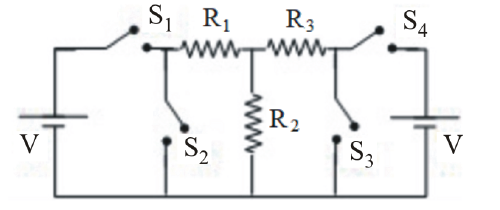
\includegraphics[width=0.85\linewidth]{Score-II - Test 18 (13 Feb 2024)-img/p1phy_n3_circuit.png}
\end{center}

\textbf{4.} A neutron with kinetic energy k = 10 MeV activates a nuclear reaction
$$n+{}^{12}\text{C}\ \to\ {}^9\text{Be}+\alpha$$
If the kinetic energy of $\alpha$-particles emerging, at an angle of $90^\circ$ w.r.t. the direction of the neutrons, is 2.21 MeV, find the threshold energy (MeV) of the reaction [Take u = 931.1 MeV]

\textbf{5.} A current I flows along a straight conductor with round cross-section. Find the flux of the Poynting vector across the lateral surface of the conductor's segment with resistance R [in SI units.] Given [I = 2A, R = 0.5$\Omega$]

\textbf{6.} There is a black body A with temperatures 3600 K. Photons having wavelength equal to the wavelength corresponding to maximum spectral radiancy of A are incident on a metal sphere having work-function 1.2 eV. The maximum kinetic energies of the electrons emitted by these photons are \ldots\ldots\ldots eV.
Take : hc = 12400 eV\AA, b = $2.88\times10^{-3}$ mK

\sectionhdr{PART-2: CHEMISTRY}
\subsectionhdr{Section-I (i): Single Correct}

\textbf{1.} Select the CORRECT statements.

(a) XeF$_2$ + H$_2$O $\longrightarrow$ 2 gaseous elemental products are formed

(b) LiNO$_3$ < NaNO$_3$ < KNO$_3$ < RbNO$_3$ < CsNO$_3$ : Solubility

(c) HgS < CuS < MnS < BaS : Solubility

(d) LiCl < CsCl < RbCl < NaCl < KCl : Solubility

\begin{qoptions}
\opt{A}{a, b}
\opt{B}{b, c}
\opt{C}{a, c}
\opt{D}{b, d}
\end{qoptions}

\textbf{2.} Give the correct order of initials True (T) or False (F) for the following statements.

(I) Quartz is extensively used as a piezoelectric material

(II) Engel's sulphur is unstable and contains S$_6$ rings arranged in the chair conformation.

(III) The reduction of violet $[\text{Cr}(\text{H}_2\text{O})_6]^{3+}$ gives bright blue $[\text{Cr}(\text{H}_2\text{O})_6]^{2+}$

(IV) Bond order of N--O bond in NO$_3^-$, is $1\tfrac13$.

\begin{qoptions}
\opt{A}{TFTF}
\opt{B}{TTFF}
\opt{C}{TTTT}
\opt{D}{FTFT}
\end{qoptions}

\textbf{3.} Vapour Pressure of solution containing 8 gm of non-volatile non-electrolyte solute in 200 gm water is 25 torr. If 2 mole of water is further added to the solution vapour pressure increases by 0.5 torr. Calculate vapour pressure of pure water

\begin{qoptions}
\opt{A}{20.22 torr}
\opt{B}{25.8 torr}
\opt{C}{28.3 torr}
\opt{D}{30 torr}
\end{qoptions}

\textbf{4.} The only incorrect information is

\begin{qoptions}
\opt{A}{In isothermal expansion of an ideal gas, internal energy of the gas remains unchanged.}
\opt{B}{In adiabatic free expansion of an ideal gas, the internal energy of gas remains unchanged.}
\opt{C}{In adiabatic free expansion of an ideal gas, the initial and final temperature of the gas remains same.}
\opt{D}{In adiabatic free expansion of a Vanderwaal gas, the initial and final temperature of gas remains same.}
\end{qoptions}

\textbf{5.} Me--CH$_2$--OH $\xrightarrow{\text{K}_2\text{Cr}_2\text{O}_7,\ \text{H}^+}$ (A) $\xrightarrow[\text{(ii) Dry distillation}]{\text{(i) Ca(OH)}_2}$ (B) $\xrightarrow{\text{NaBH}_4}$ (C) $\xrightarrow[\text{2. Mg/Et}_2\text{O}]{\text{1. HBr}}$ (D) $\xrightarrow[\text{(ii) NH}_4\text{Cl}]{\text{(i) H}_2\text{C=O}}$ (E) $\xrightarrow{\text{CrO}_3\text{ in glacial acetic acid}}$ (F)

(F) is:

\begin{qoptions}
\opt{A}{Me$_2$CH--CO$_2$H}
\opt{B}{Me$_2$CH--CH$_2$OH}
\opt{C}{Me$_2$CH--CH=O}
\opt{D}{Me$_2$CH--CH$_2$--CH$_3$}
\end{qoptions}

\textbf{6.} Incorrect statement among following is:

\begin{qoptions}
\opt{A}{All C---C bond in squaric acid dianion is of same bond length}
\opt{B}{Conjugated base of squaric acid is aromatic}
\opt{C}{Squaric acid on treatment with NaHCO$_3$ give effervescence of CO$_2$}
\opt{D}{Carbonic acid is a stronger acid than squaric acid}
\end{qoptions}

\subsectionhdr{Section-I (ii): One or more correct}

\textbf{7.} The correct increasing order(s) of pH of 0.1 M -- aqueous solution of the following compounds, at $25^\circ$C, is/are

\begin{qoptions}
\opt{A}{HCl < CH$_3$COOH < HCOOH}
\opt{B}{H$_2$SO$_4$ < HCl < H$_3$PO$_4$}
\opt{C}{CH$_3$COOH < CH$_3$COONH$_4$ < CH$_3$COONa}
\opt{D}{NH$_4$Cl < CH$_3$COONH$_4$ < NH$_3$}
\end{qoptions}

\textbf{8.} The standard boiling point of benzene (C$_6$H$_6$) is $80.1^\circ$C, then for given process C$_6$H$_6(\ell)\to$C$_6$H$_6$(g), select the correct statement(s) for this process. Given phase diagram below is for benzene:

\begin{center}
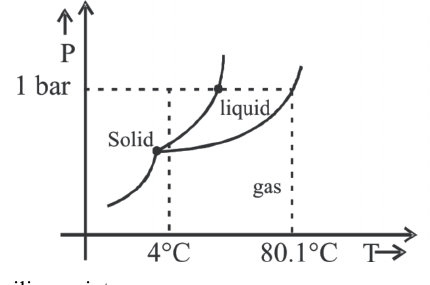
\includegraphics[width=0.6\linewidth]{Score-II - Test 18 (13 Feb 2024)-img/p2chem_q8_phase.png}
\end{center}

\begin{qoptions}
\opt{A}{$\Delta$G is zero at standard boiling point.}
\opt{B}{$\Delta$G$^\circ$ is zero at standard boiling point.}
\opt{C}{$\Delta$H$^\circ$ is positive for given process.}
\opt{D}{$\Delta$S$^\circ$ is positive for given process}
\end{qoptions}

\textbf{9.} [A] undergoes the following reactions:

\begin{center}
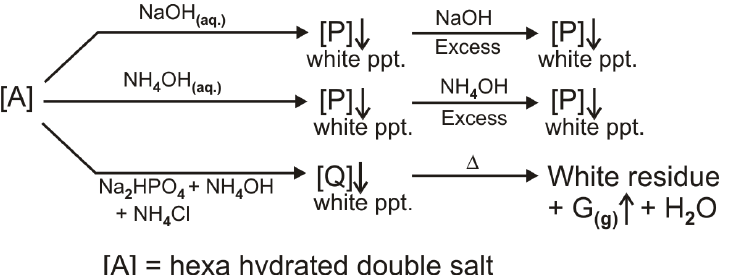
\includegraphics[width=0.9\linewidth]{Score-II - Test 18 (13 Feb 2024)-img/p2chem_q9_flowchart.png}
\end{center}

Select the correct statement:

\begin{qoptions}
\opt{A}{Metal in double salt can be extracted by electrolytic reduction of A$_{(aq.)}$}
\opt{B}{Precipitate P can be dissolved in dil. HCl}
\opt{C}{A$_{(aq.)}$ gives basic metal carbonate ppt. with (NH$_4$)$_2$CO$_3$}
\opt{D}{Aqueous solution of A gives white/off white ppt. with NaClO$_{4(aq.)}$}
\end{qoptions}

\textbf{10.} Identify reactions correctly match with their products? (options (A)--(D) are the four reaction schemes shown)

\begin{center}
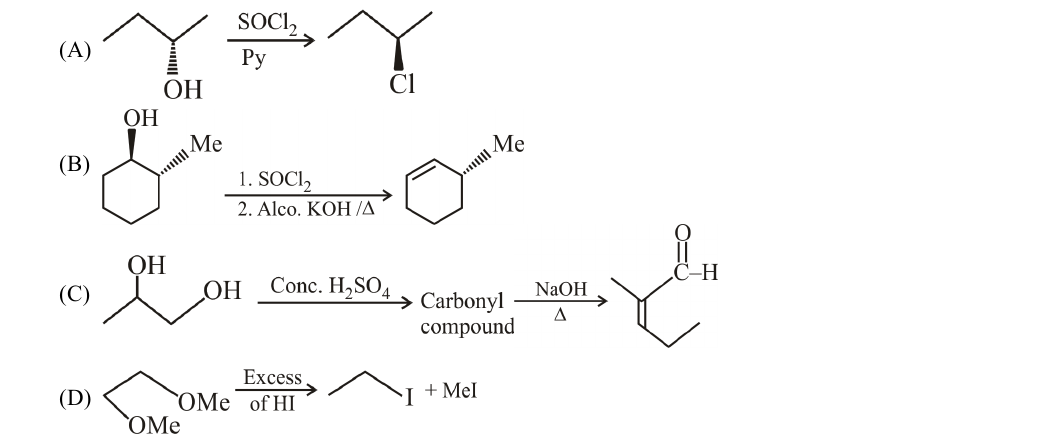
\includegraphics[width=0.85\linewidth]{Score-II - Test 18 (13 Feb 2024)-img/p2chem_q10_reactions.png}
\end{center}

\textbf{11.} Which of the following reaction form ketone as major product? (options (A)--(D) are the four reaction schemes shown)

\begin{center}
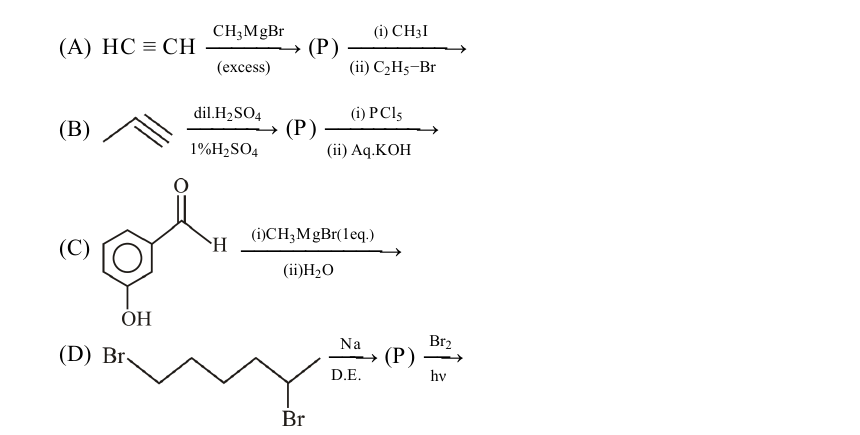
\includegraphics[width=0.75\linewidth]{Score-II - Test 18 (13 Feb 2024)-img/p2chem_q11_ketone.png}
\end{center}

\textbf{12.} Which of the following statement(s) is/are correct considering the given complexes?

(NH$_4$)$_2$[MnCl$_4$], K$_3$[Fe(CN)$_6$], O$_2$[PtF$_6$], K$_3$[CoF$_6$], Na$_3$[Co(C$_2$O$_4$)$_3$], [CoCl$_2$Br$_2$]$^{2-}$, [CoF$_3$(H$_2$O)$_3$]

\begin{qoptions}
\opt{A}{Total number of complexes in which anion part is paramagnetic \& non-planar are 6}
\opt{B}{Total number of complexes in which anionic part has plane of symmetry are 6.}
\opt{C}{The number of complex for which $\Delta$ > P [where $\Delta=\Delta_o/\Delta_{sp}/\Delta_t$] are 3}
\opt{D}{The number of complex which has stereo isomer is 1}
\end{qoptions}

\subsectionhdr{Section-II: Numerical Value}

\textbf{1.} A light source emits radiations having wavelength of 310 nm. Number of photons emitted by this source varies with time, as N = $10^{18}t^2$. (t in sec). If this light source is used to emit photoelectrons from a metal of work function 3.1 eV. Find the time (in sec.) during which the total maximum possible kinetic energy of all the emitted photoelectrones from the beginning is 1296 J.
(Use E(eV) = $\dfrac{12400}{\lambda(\text{\AA})}$, e = $1.6\times10^{-19}$ C).

\textbf{2.} The volume, in mL, of 0.02 M K$_2$Cr$_2$O$_7$ solution required to react with 0.288 g of ferrous oxalate in acidic medium is\_\_\_\_\_\_\_.
(Molar mass of Fe = 56 g mol$^{-1}$)

\textbf{3.} Number of following salts which is/are water insoluble but neither black nor white nor blue in color, is X then value of 2X.

Cu(CN)$_2$, Cu(OH)$_2$, Cu$_2$O, Cu$_3$[Fe(CN)$_6$]$_2$, Co(OH)NO$_3$, HgO.HgNH$_2$I, HgNH$_2$Cl, CuSO$_4$, Ag$_3$[Fe(CN)$_6$]

\textbf{4.} From the reaction of NiBr$_2$ and Ph$_2$EtP, it is possible to isolate green crystals of [Ni(Ph$_2$EtP)$_2$Br$_2$] which have a magnetic moment of 3.20 B.M. and red crystals of [Ni(Ph$_2$EtP)$_2$Br$_2$] which have a magnetic moment of zero. Find the total number of geometrical isomer of green and red colored complexes [Ph = C$_6$H$_5$-].

\textbf{5.} The structure of a peptide is given below.

\begin{center}
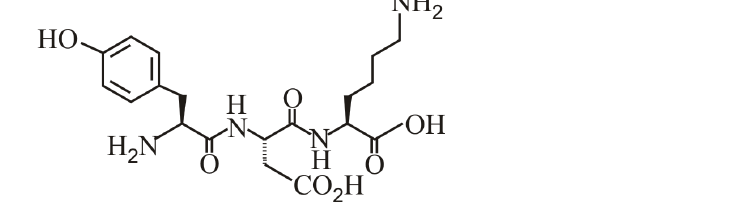
\includegraphics[width=0.85\linewidth]{Score-II - Test 18 (13 Feb 2024)-img/p2chem_n5_peptide.png}
\end{center}

If the absolute values of the net charge of the peptide at pH = 2, pH = 6, and pH = 11 are $|z_1|$, $|z_2|$ and $|z_3|$, respectively, then what is $|z_1|+|z_2|+|z_3|$?

\textbf{6.}

\begin{center}
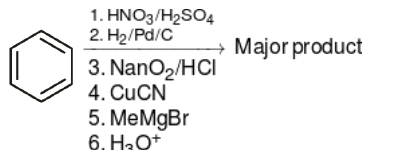
\includegraphics[width=0.4\linewidth]{Score-II - Test 18 (13 Feb 2024)-img/p2chem_n6_benzene.png}
\end{center}

Find degree of unsaturation of final major product?

\sectionhdr{PART-3: MATHEMATICS}
\subsectionhdr{Section-I (i): Single Correct}

\textbf{1.} If $\displaystyle\sum_{r=0}^{3n}a_r(x-4)^r=\sum_{r=0}^{3n}A_r(x-5)^r$ and $a_k=1\ \forall\,k\geqslant2n$ and $\displaystyle\sum_{r=0}^{3n}d_r(x-8)^r=\sum_{r=0}^{3n}B_r(x-9)^r$ and $\displaystyle\sum_{r=0}^{3n}d_r(x-12)^r=\sum_{r=0}^{3n}D_r(x-13)^r$ and $d_k=1\ \forall\,k\geqslant2n$, then the value of $\dfrac{A_{2n}+D_{2n}}{B_{2n}}$ is

\begin{qoptions}
\opt{A}{$\dfrac{4^{2n}+5^{2n}+12^{2n}+13^{2n}}{8^{2n}+9^{2n}}$}
\opt{B}{$\dfrac{5^{2n}+13^{2n}-4^{2n}-12^{2n}}{9^{2n}-8^{2n}}$}
\opt{C}{$\dfrac{5^{n}+13^{n}-4^{n}-12^{n}}{9^{n}-8^{n}}$}
\opt{D}{2}
\end{qoptions}

\textbf{2.} If $p=a+bw+cw^2$, $q=b+cw+aw^2$, and $r=c+aw+bw^2$, where $abc\neq0$ and $w=e^{i2\pi/3}$ then which of the following option is INCORRECT for all possible p, q, r?

\begin{qoptions}
\opt{A}{If p, q, r lie on the circle $|z|=2$, the triangle formed by these points is equilateral}
\opt{B}{$p^2+q^2+r^2=2(pq+qr+rp)$ (if $|p|=|q|=|r|$)}
\opt{C}{$p+q+r=0$}
\opt{D}{$p^2+q^2+r^2=a^2+b^2+c^2$}
\end{qoptions}

\textbf{3.} Three circles, each of radius 1, are packed inside an ellipse $\dfrac{x^2}{a^2}+\dfrac{y^2}{b^2}=1\ (a>b>0)$, ($2\theta=\angle ABC$), as shown in the figure. Two of these circles touch the ellipse at two points each and the middle circle touches other both circles and ellipse at the end of minor axis. A, B and C are centres of these circles.

\begin{center}
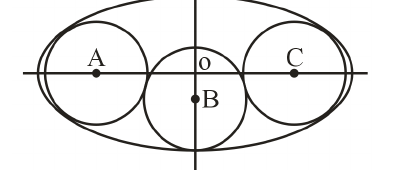
\includegraphics[width=0.55\linewidth]{Score-II - Test 18 (13 Feb 2024)-img/p3math_q3_ellipse.png}
\end{center}

If the area of ellipse is minimum, then the value of $\tan\theta$ is

\begin{qoptions}
\opt{A}{$\sqrt{27}$}
\opt{B}{$\sqrt{31}$}
\opt{C}{$\sqrt{35}$}
\opt{D}{$\sqrt{41}$}
\end{qoptions}

\textbf{4.} Given four unit vectors $\vec a,\vec b,\vec c$ and $\vec d$. The vectors $\vec a,\vec b$ and $\vec c$ are coplanar but not collinear pair by pair and vector $\vec d$ is not coplanar with vectors $\vec a,\vec b$ and $\vec c$ and $(\vec a,\vec b)=(\vec b,\vec c)=\dfrac\pi3$, $(\vec d,\vec a)=\alpha$ and $(\vec d,\vec b)=\beta$, if $(\vec d,\vec c)=\cos^{-1}(m\cos\beta+n\cos\alpha)$. For all $\alpha,\beta$ the value of $|m-n|$ is: ($(\vec x,\vec y)=\theta$ represents the angle between the vectors $\vec x$ and $\vec y$)

\begin{qoptions}
\opt{A}{2}
\opt{B}{0}
\opt{C}{1}
\opt{D}{4}
\end{qoptions}

\textbf{5.} Positive integers a, b and c are all integral power of positive integer k. If the equation $ax^2-bx+c=0$ has exactly one real solution r and this value r is less than 100, then maximum possible value of r is

\begin{qoptions}
\opt{A}{16}
\opt{B}{64}
\opt{C}{74}
\opt{D}{99}
\end{qoptions}

\textbf{6.} Two curves $x^2+2y^2+2xy-2x-2=0$ \& $x^2-y^2+2xy-2y-1=0$ intersects at A$_i$ for i = 1, 2, 3, 4. If L$_i$: x = m$_i$y denotes line OA$_i$ where O is origin and i = 1, 2, 3 \& 4. Find the equation of circle with centre $(3\Sigma m_1m_2,\ 3\Sigma m_1m_2m_3)$ \& radius $3\Sigma m_1$.

\begin{qoptions}
\opt{A}{$x^2+y^2+32x-64y+1216=0$}
\opt{B}{$x^2+y^2+32x+64y-1216=0$}
\opt{C}{$x^2+y^2+32x+64y+1216=0$}
\opt{D}{$x^2+y^2+32x-64y-1216=0$}
\end{qoptions}

\subsectionhdr{Section-I (ii): One or more correct}

\textbf{7.} Let P, Q \& R be sets defined as following:
P = \{x : x is point of discontinuities of f(x)\},
Q = \{x : x is point of non-differentiabilities of f(x)\}
R = Q -- P.
f(x) = \{x\}$\times$\{ax\}$\sin b\pi x$, where a \& b are real constants (\{.\} denotes fractional part \& I denotes set of integers), which of the following option(s) is(are) CORRECT?

\begin{qoptions}
\opt{A}{For a = $-2$ \& b = 1, the set R = I -- \{0\}}
\opt{B}{For a = $-2$ \& b = 1, the set R = $\phi$.}
\opt{C}{For P = $\phi$ \& Q = I -- \{3n : n$\in$I\}, the set of values of a's is $\left\{-\tfrac13\right\}$ \& the set of values of b's is I -- \{0\}}
\opt{D}{For a = $-\tfrac15$ \& b = $-\tfrac13$, R = \{5n : n$\in$I\} $\cup$ \{3n : n$\in$I\} -- \{15n : n$\in$I\}}
\end{qoptions}

\textbf{8.} For any $3\times3$ matrix M, let $|$M$|$ denote the determinant of M. Let A = $\begin{bmatrix}1&3&9\\2&2&10\\3&1&11\end{bmatrix}$, B = $\begin{bmatrix}10&2&2\\11&3&1\\9&1&3\end{bmatrix}$, C = $\begin{bmatrix}0&1&0\\0&0&1\\1&0&0\end{bmatrix}$. If D = $\begin{bmatrix}1&5&2\\3&7&4\\2&m&1\end{bmatrix}$ is a matrix such that $m\geqslant2$, then which of the following statements is(are) CORRECT?

\begin{qoptions}
\opt{A}{$|(AD)^{2024}| > |AD|^{2023}$}
\opt{B}{$|AD+C^2BD^{-1}| = |AD| + |CBD^{-1}|$}
\opt{C}{B = CAC and $C^3 = \begin{bmatrix}1&0&0\\0&1&0\\0&0&1\end{bmatrix}$}
\opt{D}{$C^{2024}B^2C^{2024} = AC^2A$}
\end{qoptions}

\textbf{9.} If f(x) is twice differentiable function such that $|f''(x)|\leqslant10$ for all x $\in$ [0, 5] and f(x) takes largest value at an interior point of the interval [0, 5], the value of $|f'(0)|+|f'(5)|$ cannot be

\begin{qoptions}
\opt{A}{41}
\opt{B}{43}
\opt{C}{51}
\opt{D}{57}
\end{qoptions}

\textbf{10.} Consider two parabolas P$_1$ \& P$_2$, vertices of P$_1$ \& P$_2$ are (a, b) and (a, c) respectively. Axis of symmetry of P$_1$ \& P$_2$ is x = a. y-intercepts of parabolas P$_1$ \& P$_2$ are 2024 and 2025 respectively. Length of latus rectum of P$_1$ is $\tfrac18$ and length of latus rectum of P$_2$ is $\tfrac19$. Parabola P$_1$ passes through $(\alpha_1,0)$ \& $(\alpha_2,0)$ and P$_2$ passes through $(\beta_1,0)$ and $(\beta_2,0)$ where $\alpha_1,\alpha_2,\beta_1,\beta_2\in$N (N denotes set of natural numbers) which of the following option(s) is(are) CORRECT?

\begin{qoptions}
\opt{A}{value of a is 17}
\opt{B}{value of $|b+c|$ is 864}
\opt{C}{If $\alpha_1<\alpha_2$ then value of $\alpha_1$ is 13}
\opt{D}{If $\beta_1<\beta_2$ then value of $\beta_2$ is 25}
\end{qoptions}

\textbf{11.} For real valued function which of the following statement(s) is(are) always CORRECT?

\begin{qoptions}
\opt{A}{Let f be continuous function on [0, 1] such that f(0) = 0 and f(1) = 1 and differentiable on (0, 1). For arbitrary positive real numbers m and n there exist distinct real x$_1$ and x$_2$ in [0, 1] such that $\dfrac{m}{f'(x_1)}+\dfrac{n}{f'(x_2)}=m+n$.}
\opt{B}{If f(x) is continuous at x = a and $\displaystyle\lim_{h\to0}\dfrac{f(a+2h)-2f(a+h)+f(a)}{h^2}=\lambda$ ($\lambda$ finite) then $f''(a)=\lambda$.}
\opt{C}{If f : [0, 1] $\to(0,\infty)$ then $\displaystyle\int_0^1 f^3(x)\,dx+\dfrac18\geqslant\dfrac34\left(\int_0^1 f(x)\,dx\right)^2$}
\opt{D}{If f : [0, 1] $\to(0,\infty)$ then $\displaystyle\int_0^1 f^3(x)\,dx+\dfrac1{16}\geqslant\dfrac34\int_0^1 f^2(x)\,dx$}
\end{qoptions}

\textbf{12.} For regular tetrahedron (whose edges are all equal in length) which of the following option(s) is(are) CORRECT?

\begin{qoptions}
\opt{A}{The angle between any two plane faces is $\cos^{-1}\dfrac13$.}
\opt{B}{The angle between any edge and a face not containing the edge is $\cos^{-1}\left(\sqrt{\dfrac13}\right)$.}
\opt{C}{Any two opposite edges are perpendicular to each other}
\opt{D}{The distance of any vertex from the opposite face is $\sqrt{\dfrac23}\,\ell$ : $\ell$ being length of edge.}
\end{qoptions}

\subsectionhdr{Section-II: Numerical Value}

\textbf{1.} Let x, y and z be real numbers satisfying $y-x-z=xyz$. The maximum value of the expression $p=\dfrac{2}{x^2+1}-\dfrac{2}{y^2+1}+\dfrac{3}{z^2+1}$ can be written as $\dfrac pq$ for coprime positive integers p and q. Find p + q.

\textbf{2.} For positive integer n, let $f_n(x)=\cos(x)\cos(2x)\cos(3x)\ldots\cos(nx)$. The smallest value of 'n' such that $|f_n''(0)|>2024$ is

\textbf{3.} Let $f_1(x)=\left|x-\dfrac23\right|$
$f_2(x)=\left|f_1(x)-\dfrac2{3^2}\right|$
$f_3(x)=\left|f_2(x)-\dfrac2{3^3}\right|$
$\vdots$
$f_n(x)=\left|f_{n-1}(x)-\dfrac2{3^n}\right|$

If $\displaystyle\lim_{n\to\infty}\int_{-1}^1 f_n(|x|)\,dx=\dfrac ab$ where a, b $\in$ N and H.C.F.(a, b) = 1, then the value of a + b is equal to

\textbf{4.} If $\displaystyle S(n)=\sum_{r=0}^n\dfrac1{{}^nC_r}$ and $\displaystyle P(n)=\sum_{r=1}^{n+1}\dfrac{2^r}r$, then the value of $2^{2022}\times\dfrac{S(2023)}{P(2023)}$

\textbf{5.} The number of non-empty subsets S $\subseteq\{-10,-9,-8,\ldots,8,9,10\}$ that satisfy $|S|+\min(S)\times\max(S)=0$
(min(S) is defined as smallest element in S \& max(S) is defined as greatest element in S)

\textbf{6.} A fair six-sided dice is rolled and a fair four-sided dice is rolled. What is the expected value of the sum of the numbers rolled?

\end{document}
